% siminos/spatiotemp/Examples/examReflecti.tex
% $Author: predrag $ $Date: 2021-08-02 20:53:14 -0400 (Mon, 02 Aug 2021) $

\renewcommand{\Refl}{\ensuremath{{\sigma}}} % conflict with ``symmetric''

%%%%%%%%%%%%%%%%%%%%%%%%%%%%%%%%%%%%%%%%%%%%%%%%%%%%%%%%%%%%%%%%%%
\BFIG{1.0}{bimodSaw}{}{
The $\Dn{1}$-equivariant bimodal sawtooth map of
\reffig{dscr:f_1d_symm_A} has three types of
\po s:
(a) $\Dn{1}$-fixed fixed point \cycle{C},
asymmetric fixed points pair $\{\cycle{L},\cycle{R}\}$.
(b) $\Dn{1}$-symmetric ({setwise} invariant) 2-cycle \cycle{LR},
composed of the relative cycle segment from $L$ to $R$
and its repeat from $R$ to $L$.
(c) Asymmetric 2-cycles pair $\{\cycle{LC},\cycle{CR}\}$.
~~(study \refexam{exam:Reflecti};
   continued in \reffig{dscr:f_1d_symm_b})
\authorYL{}
}{dscr:f_1d_symm_a}
%%%%%%%%%%%%%%%%%%%%%%%%%%%%%%%%%%%%%%%%%%%%%%%%%%%%%%%%%%%%%%%

%%%%%%%%%%%%%%%%%%%%%%%%%%%%%%%%%%%%%%%%%%%%%%%%%%%%%%%%%%%%%%%%%%%%%%%
\example{$\Dn{1}$-asymmetric cycles.}{ \label{exam:Reflecti} % was dscr:Reflecti
% in examDiscrete.tex, called by \Chapter{discrete}{}{World in a mirror}
% was titled "Group $\Dn{1}$ - a reflection symmetric $1d$ map"
        \index{sawtooth map}\index{map!sawtooth}             \toCB
(Continued from \refexam{exam:ReflectA})~~
	% discreteD1.mp4
	% Title:     Handwritten: a 1-dimensional fundamental domain
	% "It does not say anyplace in the Bible that if equations of motion
	% have a symmetry, solutions should have it too."
	\PC{2019-02-18}{REPLACE discreteD1.mp4, eventually.}
\toVideo{youtube.com/embed/Le5LvdDWSFQ} % uploaded 2015-01-04
    %
The $\Dn{1}$-equivariance of a map, $\Dn{1}=\{e,\Refl\}$, implies that,
in particular, if
a finite set of states ${\pS}_p=\{\ssp_n\}$ constitutes a \po\ $p$, so
does its reflection ${\pS}_{\Refl{p}}=\{\Refl\ssp_n\}$, with the same
period and the same stability properties.

Label the three regions $\pS=\{\pS_L,\pS_C,\pS_R\}$ of the bimodal
`sawtooth' map of \reffig{dscr:f_1d_symm_a}, with a 3-letter alphabet
$L$(eft), $C$(enter), and $R$(ight). This symbolic dynamics is complete
ternary dynamics, with any sequence of letters $\alphabet=\{L,C,R\}$
corresponding to an \admissible\ trajectory (`complete' means no
additional grammar rules required, see \refexam{exam:compBinSymbDyn}
below).

If $\asym$  is an \emph{asymmetric} cycle $\tilde{\pS}_\asym$, $\Refl$
maps it into the reflected cycle $\Refl\tilde{\pS}_\asym$, with no points
in common, $\tilde{\pS}_\asym\cap\Refl\tilde{\pS}_\asym=\emptyset$.
Examples are the fixed points pair $\{\cycle{L},\cycle{R}\}$ and the
2-cycles pair $\{\cycle{LC},\cycle{CR}\}$ in
\reffig{dscr:f_1d_symm_a}\,(c).
                                        \jumpBack{exam:Reflecti}
        } % end \example{exam:Reflecti}
%%%%%%%%%%%%%%%%%%%%%%%%%%%%%%%%%%%%%%%%%%%%%%%%%%%%%%%%%%%%%%%%%%%%%%%

%%%%%%%%%%%%%%%%%%%%%%%%%%%%%%%%%%%%%%%%%%%%%%%%%%%%%%%%%%%%%%%%%%%%%%%
\example{$\Dn{1}$-symmetric cycles.}{ \label{exam:ReflectiSS} % was dscr:ReflectiSS
% in examDiscrete.tex, called by \Chapter{discrete}{}{World in a mirror}
        \index{sawtooth map}\index{map!sawtooth}             \toCB
(Continued from \refexam{exam:Reflecti})~~
For $\Dn{1}$  the period of a {set-wise} symmetric cycle is even ($\nsym
= 2 \nsymf$), and the mirror image of the $\ssp_\sym$ periodic point is
reached by traversing the \rpo\ segment $\symf$  of length $\nsymf$,
$\flow{\nsymf}{\ssp_\sym} = \Refl \ssp_\sym $, see
\reffig{dscr:f_1d_symm_a}\,(b).
                                        \jumpBack{exam:ReflectiSS}
        } % end \example{Reflection symmetric 1-d maps}{exam:ReflectiSS
%%%%%%%%%%%%%%%%%%%%%%%%%%%%%%%%%%%%%%%%%%%%%%%%%%%%%%%%%%%%%%%%%%%%%%%

%%%%%%%%%%%%%%%%%%%%%%%%%%%%%%%%%%%%%%%%%%%%%%%%%%%%%%%%%%%%%%%%%%%%%%%
\example{$\Dn{1}$-invariant cycles.}{ \label{exam:ReflectiPS} % was dscr:ReflectiPS
% in examDiscrete.tex, called by \Chapter{discrete}{}{World in a mirror}
        \index{sawtooth map}\index{map!sawtooth}             \toCB

\Fix{\Group}, the set of points invariant under group action of $\Dn{1}$,
$\tilde{\pS} \cap \Refl \tilde{\pS}$, is just this fixed point $\ssp=0$,
the reflection symmetry point.

In the example at hand there is only one \Group-invariant (point-wise
invariant) orbit, the fixed point \cycle{C} at the origin, see
\reffig{dscr:f_1d_symm_a}\,(a). As reflection symmetry is the only
discrete symmetry that a map of the interval can have, this example
completes the group-theoretic analysis of 1\dmn\ maps. We shall continue
analysis of this system in \refexam{dscr:C2FundDom}, and work out the
symbolic dynamics of such reflection symmetric systems in
\refexam{exam:Symm1d}).    % was (\refsect{s-C-2-fact})
                                        \jumpBack{exam:ReflectiPS}
        } % end \example{Reflection symmetric 1-d maps}{exam:ReflectiPS
%%%%%%%%%%%%%%%%%%%%%%%%%%%%%%%%%%%%%%%%%%%%%%%%%%%%%%%%%%%%%%%%%%%%%%%

%%%%%%%%%%%%%%%%%%%%%%%%%%%%%%%%%%%%%%%%%%%%%%%%%%%%%%%%%%%%%%%%%%
\FIG{
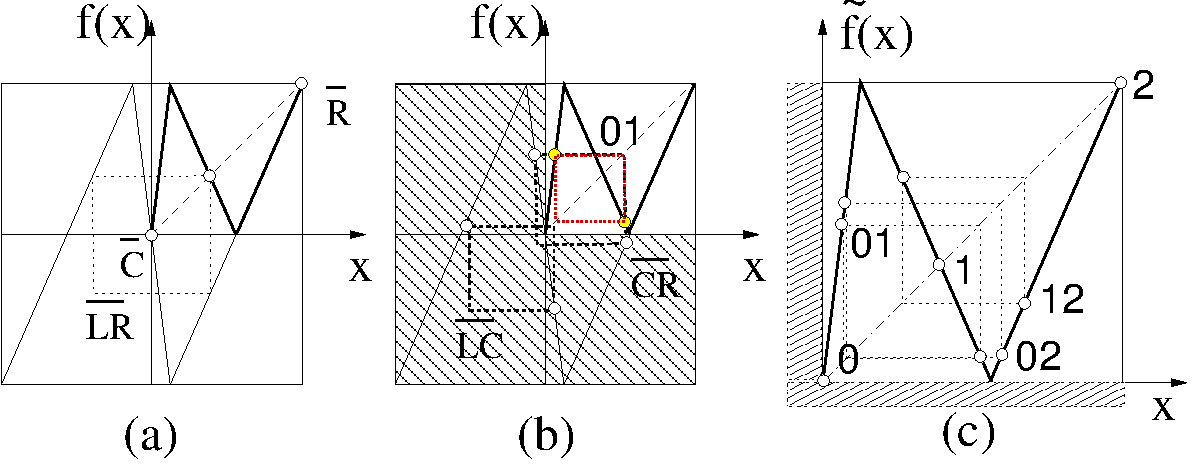
\includegraphics[width=0.95\textwidth]{bimodFund}
}{}{
The bimodal Ulam sawtooth map of \reffig{dscr:f_1d_symm_a}
with the $\Dn{1}$ symmetry $f(-\ssp)=-f(\ssp)$,
restricted to the fundamental domain.
$f(\ssp)$ is indicated by the thin line, and
fundamental domain map ${\tilde\map}({\tilde \ssp})$ by the
thick line.
(a) Boundary fixed point \cycle{C} is the fixed point \cycle{0}.
The asymmetric fixed point pair \{\cycle{L},\cycle{R}\}
is reduced to the fixed point \cycle{2},
and the full \statesp\ symmetric 2-cycle
\cycle{LR} is reduced to the fixed point \cycle{1}.
(b) The asymmetric 2-cycle pair
\{\cycle{LC},\cycle{CR}\} is reduced to 2-cycle \cycle{01}.
(c) All fundamental domain fixed points and 2-cycles.
~~(work through \refexam{dscr:C2FundDom} )
% continued in #\reffig{??}).
\authorYL{}
}{dscr:f_1d_symm_b}
%%%%%%%%%%%%%%%%%%%%%%%%%%%%%%%%%%%%%%%%%%%%%%%%%%%%%%%%%%%%%%%

%%%%%%%%%%%%%%%%%%%%%%%%%%%%%%%%%%%%%%%%%%%%%%%%%%%%%%%%%%%%%%%%%%%%%%%
\example{$\Dn{1}$ reduction to the fundamental domain.}
{ \label{dscr:C2FundDom}
% in examDiscrete.tex, called by \Chapter{discrete}{}{World in a mirror}
        \index{sawtooth map}\index{map!sawtooth}             \toCB
Consider again
the reflection-symmetric bimodal Ulam sawtooth map $f(-\ssp)=-f(\ssp)$
of \refexam{exam:Reflecti}, with symmetry group $\Dn{1}=\{{ e},\Refl\}$.
The {\statesp} $\pS = [-1,1]$
can be tiled by half-line $\tilde{\pS}=[0,1]$, and
${ \Refl}\tilde{\pS}=[-1,0]$, its image under
a reflection across $\ssp=0$ point.
The dynamics can then be restricted to the
{\em fundamental domain} $\tilde{\ssp}_k \in \tilde{\pS}=[0,1]$;
every time a trajectory leaves this interval, it is
mapped back using $\Refl$.

In \reffig{dscr:f_1d_symm_b}
% the bimodal Ulam sawtooth map
% $f(\ssp)$ is indicated by the thin line.
the fundamental
domain map ${\tilde\map}({\tilde \ssp})$
% , indicated by the thick line, %in \reffig{dscr:f_1d_symm_b},
is obtained by reflecting $\ssp < 0$ segments
of the global map $f(\ssp)$ %, \reffig{dscr:f_1d_symm_a}\,(a),
into the upper right quadrant.
${\tilde\map}$ is also bimodal and piecewise-linear,
with $\tilde{\pS} = [0,1]$ split into three regions
$\tilde{\pS} = \{\tilde{\pS}_0,\tilde{\pS}_1,\tilde{\pS}_2\}$
which we label with a 3-letter alphabet
$\tilde{\alphabet} = \{0,1,2\}$.
The symbolic dynamics is
again complete ternary dynamics, with any sequence of
letters $\{0,1,2\}$ \admissible.

However, the interpretation of the `desymmetrized'
dynamics is quite different - the multiplicity of
every \po\ is now 1, and {relative periodic segments}
of the full \statesp\ dynamics
are all \po s in the fundamental domain.
Consider \reffig{dscr:f_1d_symm_b}:

In (a)
the boundary fixed point \cycle{C} is also the fixed point \cycle{0}.
%
The asymmetric fixed point pair \{\cycle{L},\cycle{R}\}
is reduced to the fixed point \cycle{2},
and the full \statesp\ symmetric 2-cycle
\cycle{LR} is reduced to the fixed point \cycle{1}.
(b) The asymmetric 2-cycle pair
\{\cycle{LC},\cycle{CR}\} is reduced to the 2-cycle \cycle{01}.
Finally, the symmetric 4-cycle
\cycle{LCRC} is reduced to the 2-cycle \cycle{02}.
This completes the conversion from the full \statesp\ for all
fundamental domain fixed points and 2-cycles,
frame~(c).
	\PC{2019-02-18}{draw this cycle both in the full and in the
            fundamental domain.
		\\
	    in \reffig{dscr:f_1d_symm_b}\,(a) double label,
		with \cycle{0}, \cycle{1} and \cycle{2}.}
                                        \jumpBack{dscr:C2FundDom}
    } %end \example{Group $\Dn{1}$ - fundamental domain}
%%%%%%%%%%%%%%%%%%%%%%%%%%%%%%%%%%%%%%%%%%%%%%%%%%%%%%%%%%%%%%%%%%%%%%%

\renewcommand{\Refl}{\ensuremath{{s}}} % Dihedral wiki convention
